\documentclass[10pt]{article}

\usepackage[margin=0.72in]{geometry}
\usepackage{amsmath,amssymb,mathtools}
\usepackage{algorithm}
\usepackage{algpseudocode}
\usepackage{xcolor}
\usepackage{tikz}
\usepackage{graphicx}
\usetikzlibrary{arrows.meta,positioning,fit,calc}

\definecolor{algblue}{RGB}{0,70,180}
\newcommand{\unique}[1]{\textcolor{algblue}{#1}}
\newcommand{\sg}{\operatorname{sg}}
\newcommand{\R}{\mathbb{R}}
\newcommand{\diag}{\operatorname{diag}}
\newcommand{\offdiag}{\operatorname{offdiag}}

\title{Multivariate Optimization Formulations for DriftXpress Algorithms}
\author{}
\date{}

\begin{document}
\maketitle

\section*{Common notation}

Let $\mathcal D=\{(x_i,c_i)\}_{i=1}^N$, with $x_i\in[0,1]^D$, $D=784$, and
$c_i\in\{1,\ldots,C\}$, $C=6$.  For $\xi_i\sim\mathcal N(0,I_d)$,
\begin{equation}
 z_i^+=\mu_\phi(x_i)+\exp\!\left(\tfrac12\ell_\phi(x_i)\right)\odot\xi_i,
 \qquad
 z_i^-=G_\theta(\varepsilon_i,c_i),
 \qquad
 \widehat x_i=D_\psi(z_i^+).
\end{equation}

For temperature $T>0$, define $k_T(u,v)=\exp(-\lVert u-v\rVert_2/T)$.  For each
class $c$, let $\mathcal S_c$ be the fixed positive-latent support, $U_c$ its
landmarks, $W_c=K_{U_cU_c}^{-1/2}$, and
\begin{equation}
 \varphi_c(z)=W_c^{\mathsf T}k_T(U_c,z),\qquad
 A_c=\sum_{u\in\mathcal S_c}\varphi_c(u)u^{\mathsf T},\qquad
 b_c=\sum_{u\in\mathcal S_c}\varphi_c(u).
\end{equation}
The class-conditional attraction and batch repulsion fields are
\begin{align}
 m_c^+(z)&=\frac{A_c^{\mathsf T}\varphi_c(z)}{\varphi_c(z)^{\mathsf T}b_c+\epsilon},\\
 m^-(z_b;Z)&=\frac{\sum_{j\neq b}k_T(z_b,z_j)z_j}
 {\sum_{j\neq b}k_T(z_b,z_j)+\epsilon},\\
 V_b(Z,c)&=m_{c_b}^+(z_b)-m^-(z_b;Z).
\end{align}

For a batch $Z=(z_b)_{b=1}^B$, define
\begin{align}
 \mathcal D(Z,c)
 &=\frac{1}{Bd}\sum_{b=1}^B
 \left\lVert z_b-\sg\!\left(z_b+V_b(Z,c)\right)\right\rVert_2^2,\\
 \mathcal V(Z)&=\frac1d\sum_{j=1}^d
 \left[\gamma-\sqrt{\operatorname{Var}_b(Z_{bj})+\epsilon_v}\right]_+,\\
 \mathcal C(Z)&=\frac1d\left\lVert\offdiag\!\left(
 \frac{\bar Z^{\mathsf T}\bar Z}{B-1}\right)\right\rVert_F^2,\\
 \mathcal R(X,\widehat X)&=\frac{1}{BD}\lVert X-\widehat X\rVert_F^2,\\
 \mathcal K(\mu,\ell)&=\frac{1}{2B}\sum_{b=1}^B\sum_{j=1}^d
 \left(\mu_{bj}^2+e^{\ell_{bj}}-1-\ell_{bj}\right).
\end{align}

\section*{Algorithm 1: joint conditional training}

\begin{equation}
 \boxed{
 \min_{\phi,\psi,\theta}\;
 \mathbb E\!\left[
 \mathcal R(X,D_\psi(Z^+))
 +\lambda_{\mathrm{KL}}\mathcal K(\mu_\phi,\ell_\phi)
 +\lambda_{\mathrm d}^{(t)}\mathcal D(Z^-,c)
 +\lambda_{\mathrm v}\bigl(\mathcal V(Z^+)+\mathcal V(Z^-)\bigr)
 +\lambda_{\mathrm c}\bigl(\mathcal C(Z^+)+\mathcal C(Z^- )\bigr)
 \right]
 }
 \label{eq:alg1}
\end{equation}
\noindent
where
\[
 \lambda_{\mathrm d}^{(t)}=\lambda_{\mathrm d}
 \min\!\left\{1,1+3\max\!\left(0,1-\frac{t}{30}\right)\right\}.
\]
\noindent
\noindent
With the cache fixed, the objective is computationally separable:
\begin{equation}
 \mathcal L_1=\underbrace{\mathcal L_1^+(\phi,\psi)}_{\mathcal R+\lambda_{\mathrm{KL}}\mathcal K+\lambda_{\mathrm v}\mathcal V(Z^+)+\lambda_{\mathrm c}\mathcal C(Z^+)}
 +\underbrace{\mathcal L_1^-(\theta)}_{\lambda_{\mathrm d}^{(t)}\mathcal D(Z^-,c)+\lambda_{\mathrm v}\mathcal V(Z^-)+\lambda_{\mathrm c}\mathcal C(Z^-)}.
 \label{eq:alg1split}
\end{equation}
\unique{Algorithm 1 uses one loop and one optimizer object, but it is not fully joint in the computational-graph sense: $\mathcal L_1^+$ updates $(\phi,\psi)$ and $\mathcal L_1^-$ updates only $\theta$ because $Z^-=G_\theta(\varepsilon,c)$ bypasses $D_\psi$ and $\mu_\phi$.}

\begin{algorithm}[H]
\caption{Algorithm 1 training}
\begin{algorithmic}[1]
\Require $\mathcal D$, $T$, landmark count $r$, step size $\eta$, weights $\lambda$
\Ensure $(\phi,\psi,\theta)$
\State Initialize $(\phi,\psi,\theta)$; build fixed $\{U_c,W_c,A_c,b_c\}_{c=1}^C$
\For{$t=0,\ldots,T_{\mathrm{train}}$}
    \State Sample minibatch $(X,c)$ and noise $(\Xi,\varepsilon)$
    \State $Z^+\gets q_\phi(X;\Xi)$; $\widehat X\gets D_\psi(Z^+)$; $Z^-\gets G_\theta(\varepsilon,c)$
    \State Compute $V(Z^-,c)$ and $\mathcal L_1^+,\mathcal L_1^-$ from \eqref{eq:alg1split}
    \State $(\phi,\psi)\gets(\phi,\psi)-\eta\nabla_{\phi,\psi}\mathcal L_1^+$;\quad $\theta\gets\theta-\eta\nabla_\theta\mathcal L_1^-$
\EndFor
\State \Return $(\phi,\psi,\theta)$
\end{algorithmic}
\end{algorithm}

\section*{Algorithm 2: separate VAE and generator optimization}

\textbf{Stage I (VAE):}
\begin{equation}
 (\widehat\phi,\widehat\psi)\in\arg\min_{\phi,\psi}\;
 \mathbb E\!\left[
 \mathcal R(X,D_\psi(Z^+))
 +\lambda_{\mathrm{KL}}\mathcal K(\mu_\phi,\ell_\phi)
 +\lambda_{\mathrm v}\mathcal V(\mu_\phi(X))
 +\lambda_{\mathrm c}\mathcal C(\mu_\phi(X))
 \right].
 \label{eq:alg2vae}
\end{equation}

\textbf{Stage II (conditional generator):}
\begin{equation}
 \boxed{
 \widehat\theta\in\arg\min_{\theta}\;
 \mathbb E\!\left[
 \lambda_{\mathrm d}\mathcal D(G_\theta(\varepsilon,c),c)
 +\lambda_{\mathrm v}\mathcal V(G_\theta(\varepsilon,c))
 +\lambda_{\mathrm c}\mathcal C(G_\theta(\varepsilon,c))
 \right]
 }
 \quad\text{subject to }(\phi,\psi)=(\widehat\phi,\widehat\psi)\text{ fixed}.
 \label{eq:alg2gen}
\end{equation}
\noindent
\unique{The VAE is optimized first and then frozen; the second optimization updates only the conditional generator and contains no reconstruction or KL term.}

\begin{algorithm}[H]
\caption{Algorithm 2 training}
\begin{algorithmic}[1]
\Require $\mathcal D$, $T$, landmark count $r$, step size $\eta$, weights $\lambda$
\Ensure $(\widehat\phi,\widehat\psi,\widehat\theta)$
\State Initialize $(\phi,\psi)$
\For{$t=0,\ldots,T_{\mathrm{VAE}}$}
    \State Sample $(X,c)$ and $\Xi$; form $Z^+=q_\phi(X;\Xi)$ and $\widehat X=D_\psi(Z^+)$
    \State $\mathcal L_{\mathrm{VAE}}\gets$ objective \eqref{eq:alg2vae}
    \State $(\phi,\psi)\gets(\phi,\psi)-\eta\nabla_{\phi,\psi}\mathcal L_{\mathrm{VAE}}$
\EndFor
\State Freeze $(\widehat\phi,\widehat\psi)$; build fixed $\{U_c,W_c,A_c,b_c\}_{c=1}^C$
\State Initialize $\theta$
\For{$t=0,\ldots,T_{\mathrm{G}}$}
    \State Sample $(c,\varepsilon)$; set $Z^-\gets G_\theta(\varepsilon,c)$
    \State $\mathcal L_{\mathrm{G}}\gets$ objective \eqref{eq:alg2gen}
    \State $\theta\gets\theta-\eta\nabla_\theta\mathcal L_{\mathrm{G}}$
\EndFor
\State \Return $(\widehat\phi,\widehat\psi,\theta)$
\end{algorithmic}
\end{algorithm}

\section*{Algorithm 3: fully joint training with re-encoded drift}

Define
\begin{equation}
 z_i^-=G_\theta(\varepsilon_i,c_i),\qquad
 x_i^-=D_\psi(z_i^-),\qquad
 \widetilde z_i^-=\mu_\phi(x_i^-).
\end{equation}
The optimization problem is
\begin{equation}
 \boxed{
 \min_{\phi,\psi,\theta}\;
 \mathbb E\!\left[
 \mathcal R(X,D_\psi(Z^+))
 +\lambda_{\mathrm{KL}}\mathcal K(\mu_\phi,\ell_\phi)
 +\lambda_{\mathrm d}\mathcal D(\widetilde Z^-,c)
 +\lambda_{\mathrm v}\bigl(\mathcal V(\mu_\phi(X))+\mathcal V(\widetilde Z^- )\bigr)
 +\lambda_{\mathrm c}\bigl(\mathcal C(\mu_\phi(X))+\mathcal C(\widetilde Z^- )\bigr)
 \right]
 }
 \label{eq:alg3}
\end{equation}
\noindent
\unique{Algorithm 3 is fully joint: drift is evaluated after decode--re-encode, so its gradient traverses $\widetilde Z^-\leftarrow D_\psi\leftarrow G_\theta$ and $\widetilde Z^-\leftarrow\mu_\phi$. No additional cycle loss is used.}

\begin{algorithm}[H]
\caption{Algorithm 3 training}
\begin{algorithmic}[1]
\Require $\mathcal D$, $T$, landmark count $r$, step size $\eta$, weights $\lambda$
\Ensure $(\phi,\psi,\theta)$
\State Initialize $(\phi,\psi,\theta)$; build fixed $\{U_c,W_c,A_c,b_c\}_{c=1}^C$
\For{$t=0,\ldots,T_{\mathrm{train}}$}
    \State Sample $(X,c)$ and $(\Xi,\varepsilon)$
    \State $Z^+\gets q_\phi(X;\Xi)$; $\widehat X\gets D_\psi(Z^+)$
    \State $Z^-\gets G_\theta(\varepsilon,c)$; $X^-\gets D_\psi(Z^-)$; $\widetilde Z^-\gets\mu_\phi(X^-)$
    \State Compute $V(\sg(\widetilde Z^-),c)$ and $\mathcal L_t$ from \eqref{eq:alg3}
    \State $(\phi,\psi,\theta)\gets(\phi,\psi,\theta)-\eta\nabla_{\phi,\psi,\theta}\mathcal L_t$
\EndFor
\State \Return $(\phi,\psi,\theta)$
\end{algorithmic}
\end{algorithm}

\section*{Loss-to-parameter flow}

\begin{figure}[H]
\centering
\resizebox{\linewidth}{!}{%
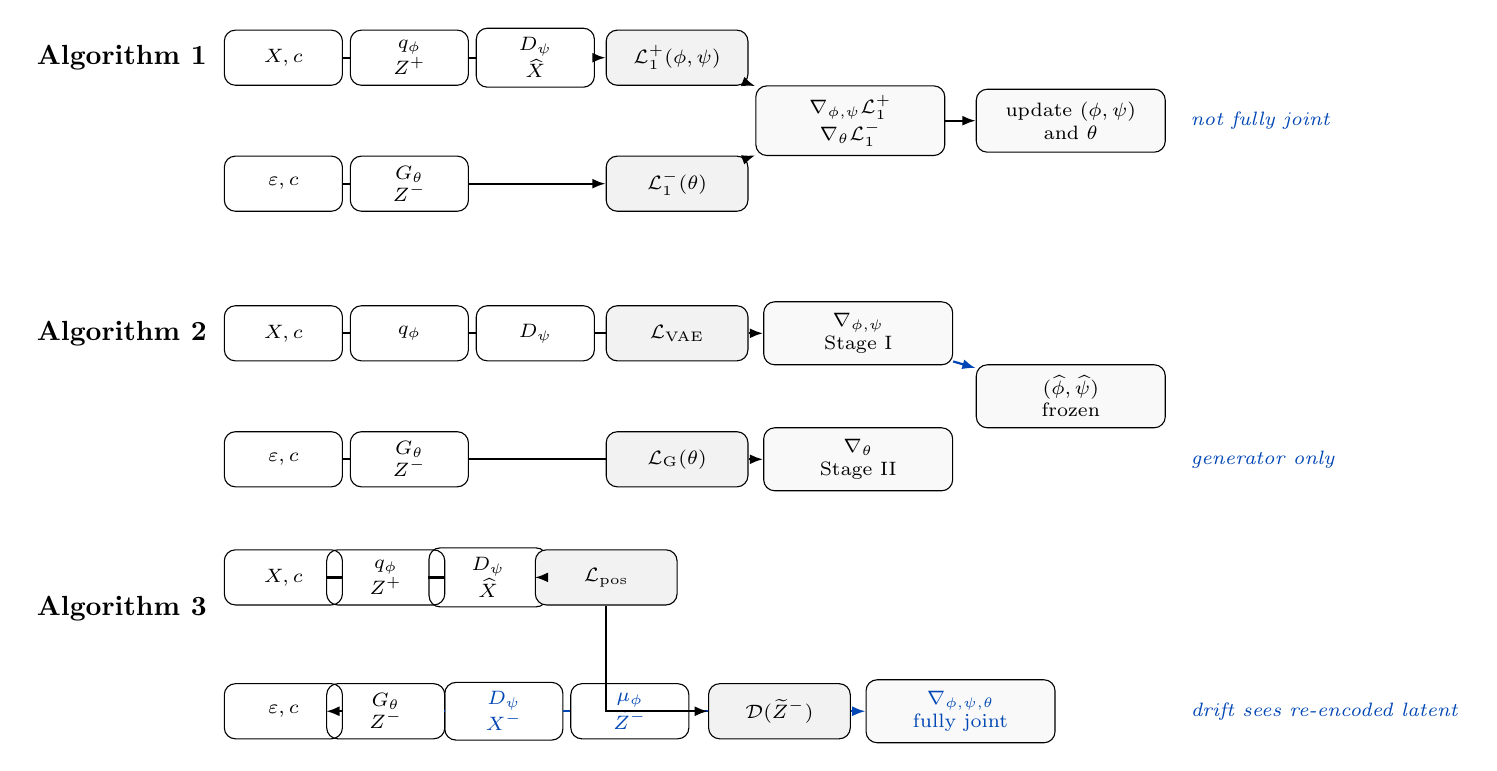
\begin{tikzpicture}[
  block/.style={draw, rounded corners, align=center, minimum width=15mm, minimum height=7mm, font=\scriptsize},
  loss/.style={draw, rounded corners, align=center, fill=gray!10, minimum width=18mm, minimum height=7mm, font=\scriptsize},
  update/.style={draw, rounded corners, align=center, fill=gray!5, minimum width=24mm, minimum height=8mm, font=\scriptsize},
  arrow/.style={-{Latex[length=1.7mm]}, thick},
  bluearrow/.style={-{Latex[length=1.7mm]}, thick, algblue}
]
% Algorithm 1: one loop, two disconnected gradient blocks.
\node[anchor=east, font=\bfseries] (a1label) at (1.35,8.3) {Algorithm 1};
\node[block] (a1data) at (2.2,8.3) {$X,c$};
\node[block] (a1enc) at (3.8,8.3) {$q_\phi$\\$Z^+$};
\node[block] (a1dec) at (5.4,8.3) {$D_\psi$\\$\widehat X$};
\node[loss] (a1pos) at (7.2,8.3) {$\mathcal L_1^+(\phi,\psi)$};
\node[block] (a1noise) at (2.2,6.7) {$\varepsilon,c$};
\node[block] (a1gen) at (3.8,6.7) {$G_\theta$\\$Z^-$};
\node[loss] (a1neg) at (7.2,6.7) {$\mathcal L_1^-(\theta)$};
\node[update] (a1update) at (9.4,7.5) {$\nabla_{\phi,\psi}\mathcal L_1^+$\\$\nabla_\theta\mathcal L_1^-$};
\node[update] (a1params) at (12.2,7.5) {update $(\phi,\psi)$\\and $\theta$};
\draw[arrow] (a1data) -- (a1enc) -- (a1dec) -- (a1pos);
\draw[arrow] (a1noise) -- (a1gen) -- (a1neg);
\draw[arrow] (a1pos) -- (a1update);
\draw[arrow] (a1neg) -- (a1update);
\draw[arrow] (a1update) -- (a1params);
\node[anchor=west, font=\scriptsize, algblue] at (13.6,7.5) {\textit{not fully joint}};

% Algorithm 2: two sequential optimizations.
\node[anchor=east, font=\bfseries] (a2label) at (1.35,4.8) {Algorithm 2};
\node[block] (a2data) at (2.2,4.8) {$X,c$};
\node[block] (a2enc) at (3.8,4.8) {$q_\phi$};
\node[block] (a2dec) at (5.4,4.8) {$D_\psi$};
\node[loss] (a2vae) at (7.2,4.8) {$\mathcal L_{\mathrm{VAE}}$};
\node[update] (a2vaeup) at (9.5,4.8) {$\nabla_{\phi,\psi}$\\Stage I};
\node[block] (a2noise) at (2.2,3.2) {$\varepsilon,c$};
\node[block] (a2gen) at (3.8,3.2) {$G_\theta$\\$Z^-$};
\node[loss] (a2g) at (7.2,3.2) {$\mathcal L_{\mathrm G}(\theta)$};
\node[update] (a2gup) at (9.5,3.2) {$\nabla_\theta$\\Stage II};
\node[update] (a2frozen) at (12.2,4.0) {$(\widehat\phi,\widehat\psi)$\\frozen};
\draw[arrow] (a2data) -- (a2enc) -- (a2dec) -- (a2vae) -- (a2vaeup);
\draw[arrow] (a2noise) -- (a2gen) -- (a2g) -- (a2gup);
\draw[bluearrow] (a2vaeup) -- (a2frozen);
\node[anchor=west, font=\scriptsize, algblue] at (13.6,3.2) {\textit{generator only}};

% Algorithm 3: a connected decode--re-encode gradient path.
\node[anchor=east, font=\bfseries] (a3label) at (1.35,1.3) {Algorithm 3};
\node[block] (a3data) at (2.2,1.7) {$X,c$};
\node[block] (a3enc) at (3.5,1.7) {$q_\phi$\\$Z^+$};
\node[block] (a3decpos) at (4.8,1.7) {$D_\psi$\\$\widehat X$};
\node[loss] (a3pos) at (6.3,1.7) {$\mathcal L_{\mathrm{pos}}$};
\node[block] (a3noise) at (2.2,0.0) {$\varepsilon,c$};
\node[block] (a3gen) at (3.5,0.0) {$G_\theta$\\$Z^-$};
\node[block] (a3dec) at (5.0,0.0) {\unique{$D_\psi$}\\\unique{$X^-$}};
\node[block] (a3reenc) at (6.6,0.0) {\unique{$\mu_\phi$}\\\unique{$\widetilde Z^-$}};
\node[loss] (a3loss) at (8.5,0.0) {$\mathcal D(\widetilde Z^-)$};
\node[update] (a3up) at (10.8,0.0) {\unique{$\nabla_{\phi,\psi,\theta}$}\\\unique{fully joint}};
\draw[arrow] (a3data) -- (a3enc) -- (a3decpos) -- (a3pos);
\draw[arrow] (a3noise) -- (a3gen);
\draw[bluearrow] (a3gen) -- (a3dec) -- (a3reenc) -- (a3loss) -- (a3up);
\draw[arrow] (a3pos) |- (a3loss);
\node[anchor=west, font=\scriptsize, algblue] at (13.6,0.0) {\textit{drift sees re-encoded latent}};
\end{tikzpicture}%
}
\caption{Loss-to-parameter flow. Algorithm 1 has two disconnected gradient blocks despite using one optimizer loop; Algorithm 2 separates VAE and generator stages; Algorithm 3 connects the generated latent to all three parameter blocks through decode--re-encode. Stop-gradient targets do not block gradients through the differentiable first arguments.}
\end{figure}

\end{document}
